%
% File acl2014.tex
%
% Contact: giovanni.colavizza@epfl.ch
%%
%% Based on the style files for ACL-2013, which were, in turn,
%% Based on the style files for ACL-2012, which were, in turn,
%% based on the style files for ACL-2011, which were, in turn, 
%% based on the style files for ACL-2010, which were, in turn, 
%% based on the style files for ACL-IJCNLP-2009, which were, in turn,
%% based on the style files for EACL-2009 and IJCNLP-2008...

%% Based on the style files for EACL 2006 by 
%%e.agirre@ehu.es or Sergi.Balari@uab.es
%% and that of ACL 08 by Joakim Nivre and Noah Smith

\documentclass[11pt]{article}
\usepackage{acl2014}
\usepackage{times}
\usepackage{url}
\usepackage{latexsym}
\usepackage{graphicx}	% For figure environment
\usepackage{booktabs} % For tables
% \usepackage{hyperref}

%\setlength\titlebox{5cm}

% You can expand the titlebox if you need extra space
% to show all the authors. Please do not make the titlebox
% smaller than 5cm (the original size); we will check this
% in the camera-ready version and ask you to change it back.


\title{Enron Emails Data-Set}

\author{Sami Ben Hassen \\
  {sami.benhassen@epfl.ch\\\tt237898} \\\And
  Firas Kanoun \\
  {firas.kanoun@epfl.ch\\\tt250235} \\\And
Ali Fessi \\
{ali.fessi@epfl.ch\\\tt247570} \\}

\date{}

\begin{document}
\maketitle
\begin{abstract}
  In 2000, Enron\cite{ENRON} was one of the largest companies in the United States. Its stock kept soaring higher and higher day by day. By 2002, it had collapsed into bankruptcy due to widespread corporate fraud. In the resulting Federal investigation, a significant amount of typically confidential information entered into the public record, including around 500.000 emails and detailed financial data for top executives.
  Getting access to an email database without violating user privacy is close to impossible. The fall of Enron gave us the opportunity to dive into the detailed analysis of emails and how people use them.
  During this project, we'll try to investigate this data-set and try to answer the research questions we came up with below.
\end{abstract}

\section{Credits}

This document is the result of our project for the class "Applied Data Analysis" also known by its code CS-401 at EPFL under the supervision of the Teaching Assistant for the class Nuno Miguel Mota Gon\c{c}alves.

The Data-Set that we are working on was collected and prepared first by the CALO Project\cite{CALO}. Later, it was purchased by Leslie Kaelbling\cite{Leslie} at MIT. And now it is being distributed by CMU\cite{CMU} as a resource for researchers who are interested in improving current email tools, or understanding how email is currently used.

\section{Introduction}

During this project, we'll try to investigate this data-set and try to answer the research questions we came up with.
In section \ref{Data Exploration} we will explore our data: we will discuss the time at which people tend to send emails, people who send the most number of emails at this particular company and finally we'll take a look at the subjects of the emails and their content. In section \ref{Network Analysis} we will analyze the data-set as a social network. After discussing the above we will dive into more interesting research: we will create machine learning models that will classify emails as spam or ham. This a great opportunity to train such algorithms since email data-sets are very hard to come by (for privacy reasons). We will then end this paper by showing the results of some supervised and unsupervised models capable of finding corrupted individuals inside a company given that we cannot mention Enron without the words fraud or manipulation coming up.

\section{Data Exploration}\label{Data Exploration}

The Data-Set is represented as a list of folders. Each folder contains the Mail-Box of an employee. Therefore each folder contains a number of sub-folders representing for example inbox, outbox... We managed to compile everything in a nice pandas data frame which helped us in our data exploration.
\subsection{Time is money}
In this part of the project we explored different times people tend to send emails inside the company and showed how valuable time in e-mails can be in finding information about the company.

\begin{figure}[htbp]
  \centering
  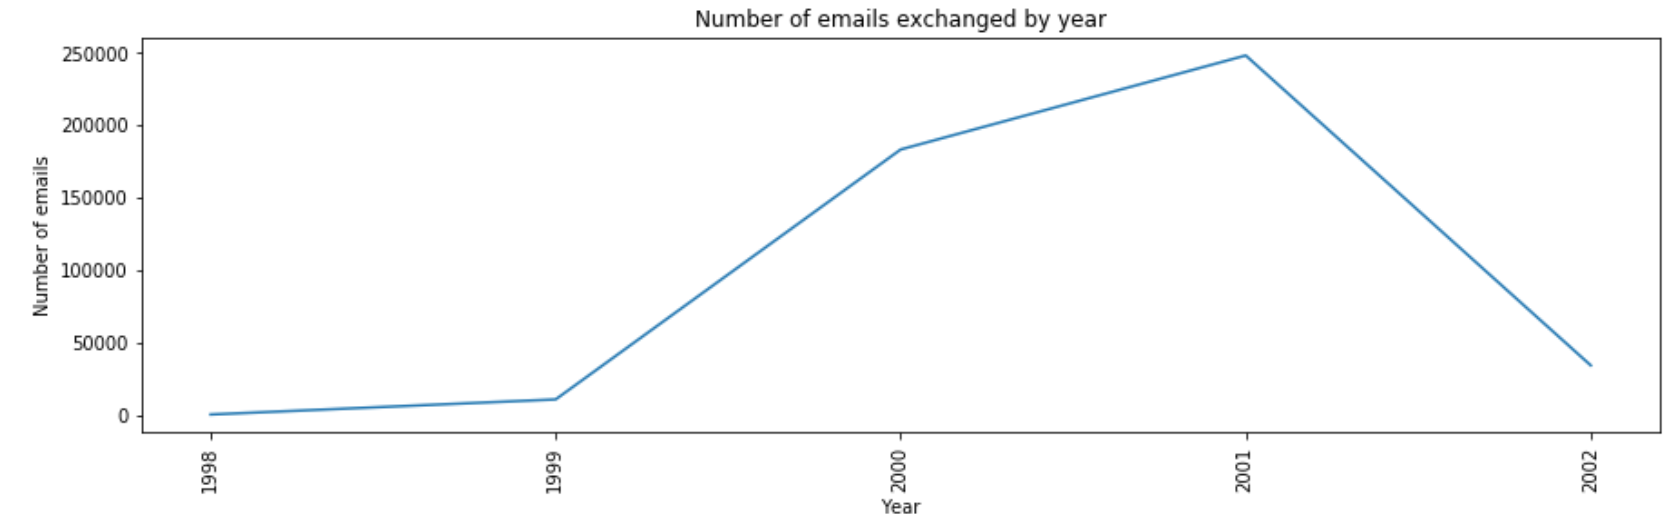
\includegraphics[width=\columnwidth]{images/emails_year.png}
  \vspace{-7mm}
  \caption{Number of emails exchanged by year.}
  \vspace{-3mm}
  \label{fig:emails_year}
\end{figure}

From the yearly graph (Fig.\ref{fig:emails_year}), we can see that the bankruptcy happened at the very beginning of the year of 2002 since the number of emails drastically decreased. If it had been towards the end we would have had more emails exchanged that year.
Checking with Wikipedia\cite{ENRON_Scandal} we find that in "Dec. 2, 2001: Enron files for Chapter 11 bankruptcy protection".

A look at the number of emails sent by hour (Fig.\ref{fig:emails_hour}) and we get the exact schedule in the day of the employees. We can confidently say that they start their day at 8AM and finish at 6PM with a one hour break at noon.
They are quite productive at 10AM and reach their highest productivity at 4PM before people start leaving. This doesn't apply to only ENRON employees though. Studies that have explored productivity in different countries around the world have shown similar productivity patterns\cite{pipedrive}. 

\begin{figure}[htbp]
  \centering
  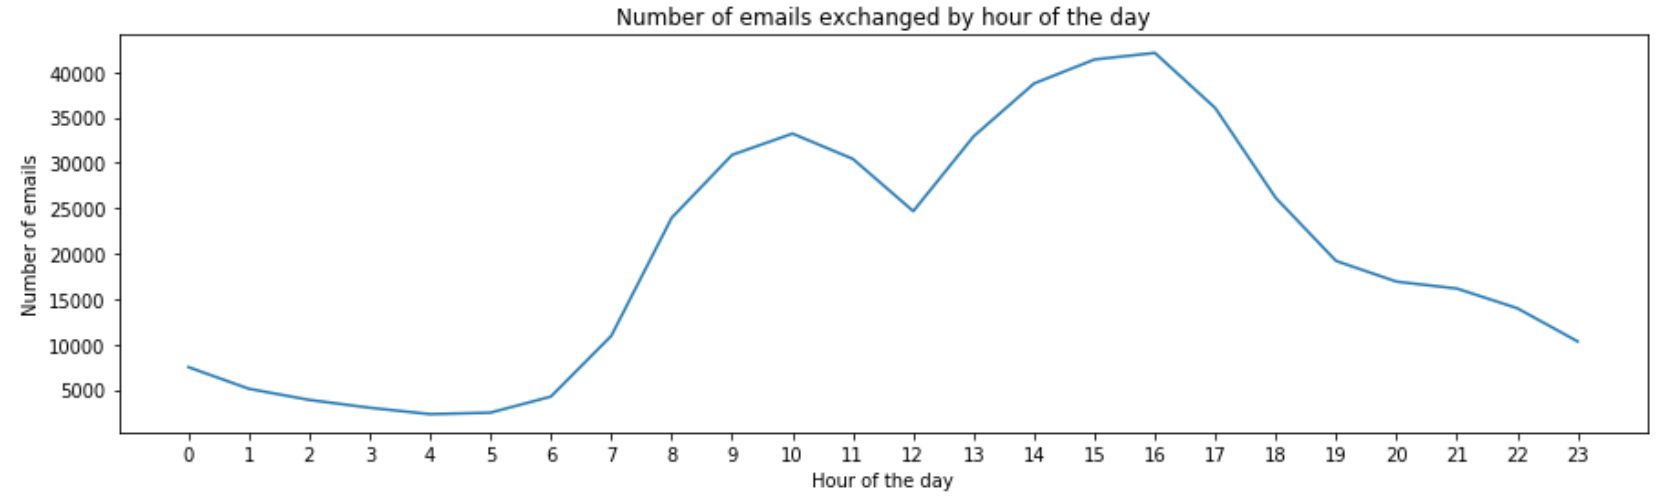
\includegraphics[width=\columnwidth]{images/emails_hour.png}
  \vspace{-7mm}
  \caption{Number of emails exchanged by hour of the day.}
  \vspace{-3mm}
  \label{fig:emails_hour}
\end{figure}


\subsection{Diving into the content}
Taking a deeper look to examine the actual content of all these emails and removing some obvious stop words (Fig.\ref{fig:subject_content}) we find out that the most used words within this company are usually part of the following categories:
\vspace{-3mm}
\begin{itemize}
\item Meetings and time updates : report, date, hour, ahead, codesite, meeting, conference, start, request, call...
\vspace{-3mm}
\item The field the company is working in: gaz, power, energy...
\vspace{-3mm}
\item The years during which the company has been more active: 2000 and 2001.
\end{itemize}

\vspace{-3mm}
\begin{figure}[htbp]
  \centering
  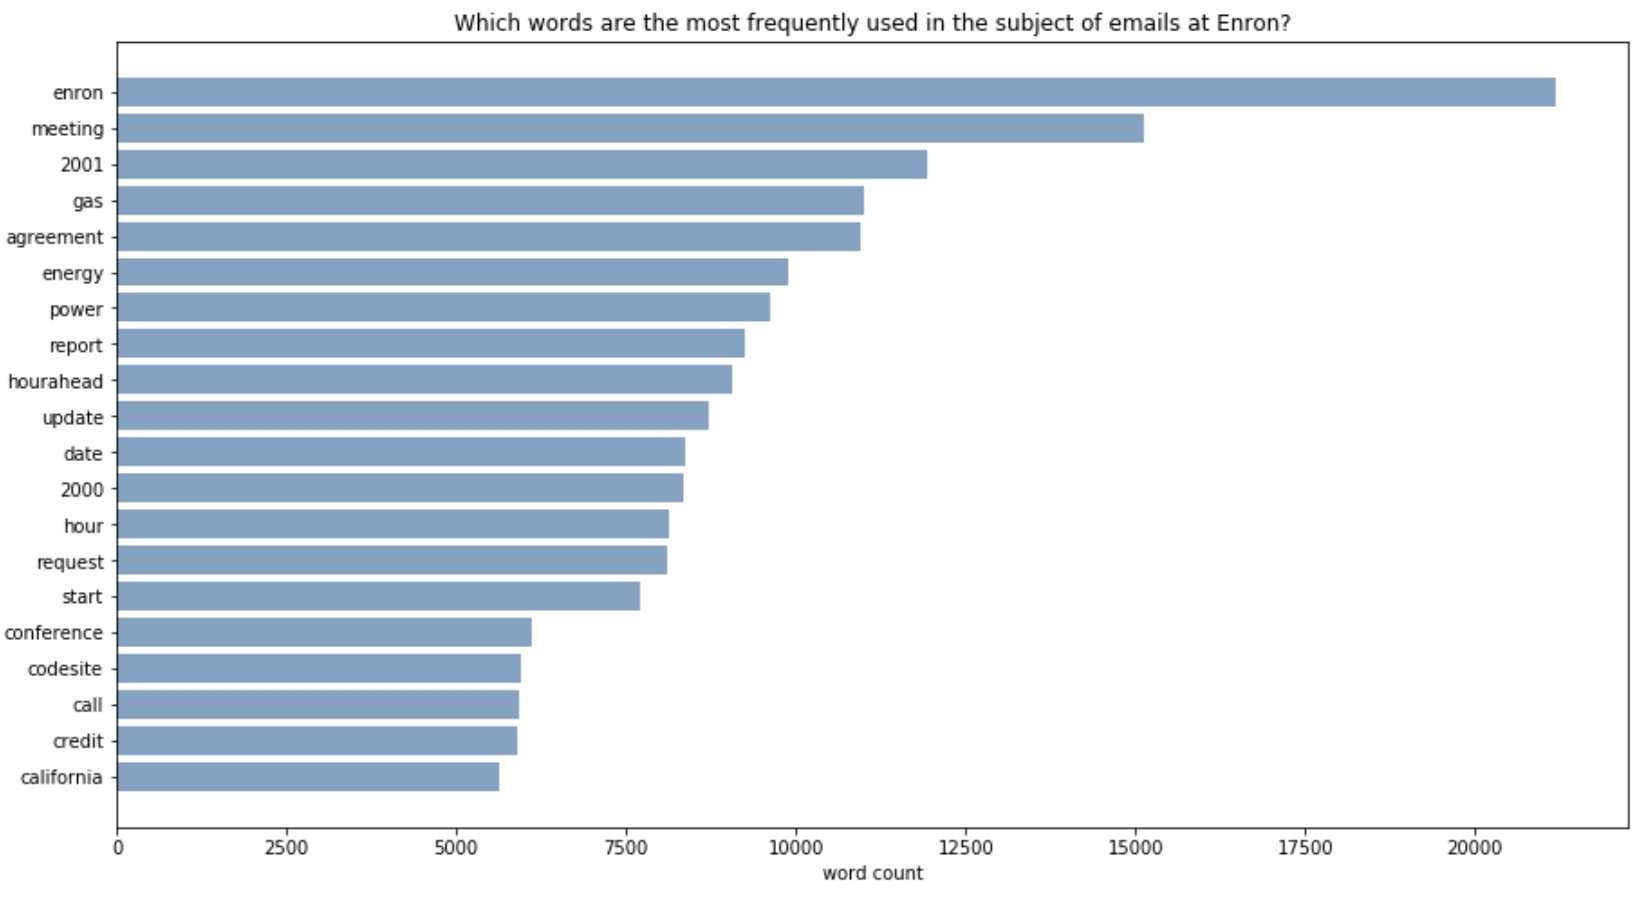
\includegraphics[width=\columnwidth]{images/subject_content.png}
  \vspace{-7mm}
  \caption{TOP Words used in the subject at ENRON}
  \vspace{-3mm}
  \label{fig:subject_content}
\end{figure}

\section{Network Analysis}\label{Network Analysis}

For this part we will create a graph having as nodes as the name of employees and the connection between them as edges. 

\begin{figure}[htbp]
  \centering
  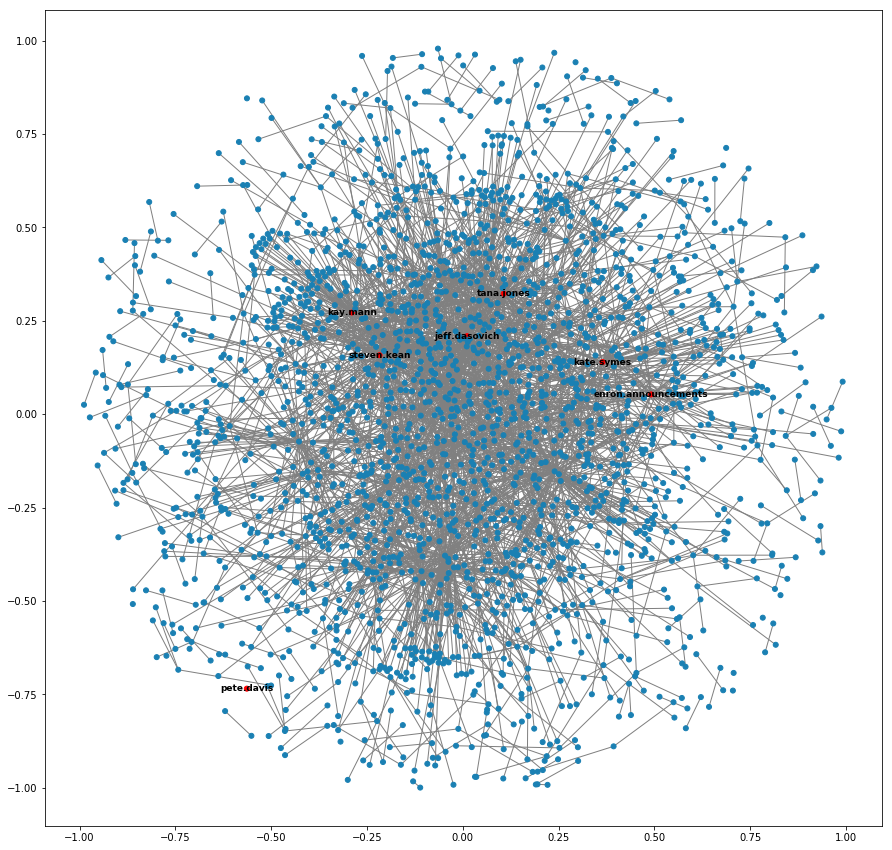
\includegraphics[width=\columnwidth]{images/social_network.png}
  \vspace{-7mm}
  \caption{The Social Network at ENRON}
  \vspace{-3mm}
  \label{fig:social_network}
\end{figure}
From Fig.\ref{fig:social_network} we can see that the most influential people are more or less in the center of this network, Nodes that are very far away from the center are likely to represent email addresses that are used as proxy like `pete.davis` which was used for auto-generated emails\cite{employee_position}. This is why we need to look at the centrality which will give us a more in depth look at the connections within the firm.

\begin{figure}[htbp]
  \centering
  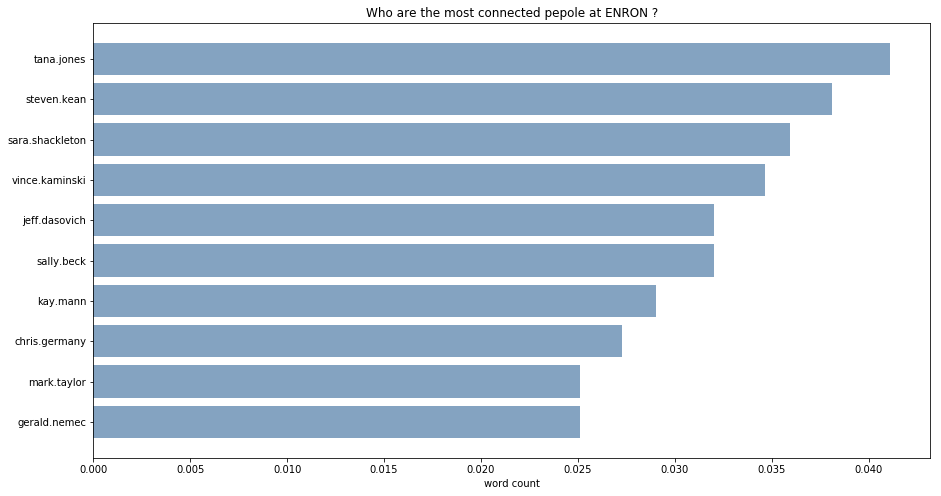
\includegraphics[width=\columnwidth]{images/most_connected.png}
  \vspace{-7mm}
  \caption{Most connected people at ENRON}
  \vspace{-3mm}
  \label{fig:most_connected}
\end{figure}

Among the most central people we find : Steven Kean which was the Vice President and Chief of Staff and Vince Kaminski as the Risk Management Head \cite{employee_position} which explains the fact that they are one of the most connected employees.

\section{SPAM Detection}\label{SPAM Detection}
\subsection{Data Acquisition}
To train a classifier for SPAM detection we had to find a source of SPAM emails we could use. We have found "SpamAssassin"\cite{spamassassin} and "HoneyPot" which are sources that provide these type of emails. Some of these emails have been mixed with our ENRON data-Set and were made available publicly\cite{spamham}. Again here the data is provided as text files inside folders and sub-folders so we did the same thing as in the data exploration part and we ended up with a balanced data frame that has 30.000 emails. 
\subsection{Train Machine Learning Models}
After cleaning up the email contents, transforming the words into vectors and applying different machine learning models we get the results displayed in table \ref{tab:results_spam}:

\begin{table}[htb]
\centering
\begin{tabular}{|l|r|} 
\cline{2-2}
\multicolumn{1}{l|}{}      & Accuracy  \\ 
\hline
\textbf{Linear SVM}  & \textbf{0.989948	}  \\ 
\hline
SGD Classifier &	0.984681\\ 
\hline
Naive Bayesian Multinomial &	0.986802\\ 
\hline
Logistic Regression	 & 0.982977\\ 
\hline
Extra Trees	& 0.973425\\ 
\hline
Random Forest	& 0.973754\\ 
\hline
AdaBoost	& 0.972014\\ 
\hline
Extra Forest & 	0.944377\\ 
\hline
k-Nearest Neighbors & 	0.785367\\ 
\hline

\end{tabular}
 \caption{Different ML algorithms results.}
    \label{tab:results_spam}
\end{table}

We can clearly see that Linear SVM, with a great accuracy of \textbf{98.99\%}, is the best model among the ones we have tested.




\section{Fraud Detection}\label{Fraud Detection}
\subsection{Building the financial data}
This part of the project shows how hard it could be to fetch and compile clean usable data.

Since the scandal, people have actually managed to collect a lot of the company's and employees' financial information that was publicly available. There is a pdf of this information available on findlaw\cite{findlaw}.

After scrapping these pdf pages and organizing them in a data frame, we tried to find matches between employees in both data-sets.

Below is a list of the interesting features we have added from the e-mails data set, the whole list is available in the notebook: 
\vspace{-3mm}
\begin{itemize}
\item The number of emails sent to POIs
\vspace{-3mm}
\item The number of emails received from POIs.
\vspace{-3mm}
\item The Stress Score, representing how many words denoting fear employees used in their emails.
\end{itemize}

\vspace{-7mm}
\begin{figure}[htbp]
  \centering
  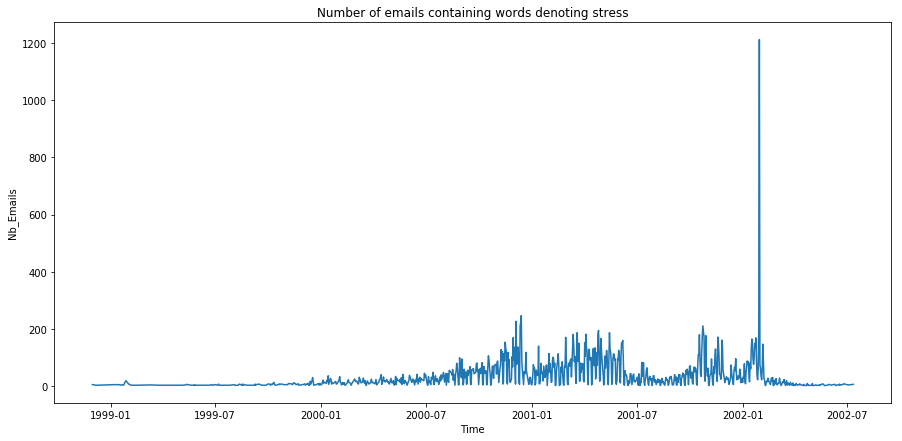
\includegraphics[width=\columnwidth]{images/stressscore.png}
  \vspace{-7mm}
  \caption{The stress score at ENRON}
  \vspace{-3mm}
  \label{fig:stressscore}
\end{figure}

Interestingly, looking at Fig.\ref{fig:stressscore} we notice that the "Stress Score" is starting to rise on July 2000, while the stock has started to decrease on January 2001. It's amazing to see that the content of e-mails gave us such an important insight 6 months before the public started to suspect a strange behaviour from the management, which was the idea behind adding this feature to our models.

Finally, we used an article from usatoday\cite{usatoday} that provides a list of all the people involved in the scandal. We extracted the names of these employees that either reached a settlement with the government, pleaded guilty or testified in exchange of persecution immunity. We labeled them as POIs (People Of Interest) and used this label as the target of our models.


\subsection{Supervised Learning Models}
We have noticed that our data-set is heavily unbalanced, containing a ratio of only 0.14 of POIs which makes it quite hard for some machine learning models to achieve good results. After looking up different methods\cite{analyticsvidhya} to overcome this problem, below are the best that have worked for us:
\subsubsection{Over-Sampling}
Over-Sampling increases the number of instances in the minority class by replicating them in order to present a higher representation of the minority class in the sample. We therefore duplicated 3 times the rows of POIs in our training set. Table.\ref{tab:Over-Sampling} shows the results.

\begin{table}[htb]
\centering
\begin{tabular}{|l|r|l|l|} 
\cline{2-4}
\multicolumn{1}{l|}{}      & Precision & Recall & F\_Score   \\ 
\hline
\textbf{KNN} &	\textbf{0.82} &	\textbf{0.82} &	\textbf{0.82} \\ 
\hline
Multi.NB  &	0.500 &	0.277 &	0.357 \\ 
\hline
SVM &	0.500 &	0.277 &	0.357 \\ 
\hline
Linear SVM &	0.500 &	0.277 &	0.357\\
\hline
RBF SVM &	0.500 &	0.277 &	0.357 \\ 
\hline
L.Regression	 &0.500 &	0.277 &	0.357 \\ 
\hline
SGD Class. &	0.48 &	0.471 &	0.45 \\ 
\hline
\end{tabular}
 \caption{Different ML algorithms results after Over-Sampling.}
    \label{tab:Over-Sampling}
\end{table}

\subsubsection{Boosting-Based Approach and Decision Trees}

Boosting is an ensemble technique to combine weak learners to create a strong learner that can make accurate predictions. Boosting starts out with a base classifier / weak classifier that is prepared on the training data.
After each iteration, the new classifier places more weight to those cases which were incorrectly classified in the last round.
We also know that decision trees are not affected too much by unbalanced data so we thought it was a good idea to use them.

Table.\ref{tab:boosting} shows the results of some decision trees and boosting ML algorithms.

Fig.\ref{fig:confusion} shows the confusion matrix of the applied model on the test set.
\begin{table}[htb]
\centering
\begin{tabular}{|l|r|l|l|} 
\cline{2-4}
\multicolumn{1}{l|}{}      & Precision & Recall & F\_Score   \\ 
\hline
\textbf{Extra Forest} &	\textbf{0.833} &	\textbf{0.952} &	\textbf{0.875}	 \\ 
\hline
\textbf{Extra Trees}  &	\textbf{0.833} &	\textbf{0.952} &	\textbf{0.875} \\ 
\hline
Random Forest &	0.5 &	0.38 &	0.431 \\ 
\hline
AdaBoost &	0.754 &	0.73 &	0.74\\
\hline

\end{tabular}
 \caption{Different Decision Trees and Boosting-Based ML algorithms results without oversampling}
    \label{tab:boosting}
\end{table}
\vspace{-4mm}



\begin{figure}[htbp]
  \centering
  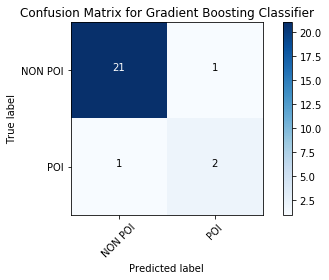
\includegraphics[width=\columnwidth]{images/confusion_matrix.png}
  \vspace{-7mm}
  \caption{Confusion Matrix for Extra Forest Classifier.}
  \vspace{-3mm}
  \label{fig:confusion}
\end{figure}

\subsection{Unsupervised Learning Models}
For this part we decided not to use any prior knowledge about employees inside Enron. We thought that executives sharing comparable salaries, bonuses and e-mails content share somehow similar responsibilities.  We therefore used K-MEANS \cite{kmeans} algorithm to perform this unsupervised task and try to classify people as corrupted or not.
We started by building two clusters as we want to resolve a classification problem. We then ran our algorithm in two dimensions by selecting two features which gave us some encouraging results that can still be improved.  We then selected the 16-most useful  features and were positively surprised to see that without any knowledge of the scandal and despite the very low amount of data we had, our model was able to give astonishing prediction results. It was able to accuse of fraud the two main responsible of the scandal Lay Kenneth : founder, CEO and Chairman of Enron Corporation for most of its existence and Jeffrey Skilling : CEO of Enron Corporation during the case.

Table.\ref{tab:unsupervised} shows the results
\begin{table}[htb]
\centering
\begin{tabular}{|l|r|l|l|} 
\hline
Accuracy & Precision & Recall & F\_Score  \\ 
\hline
0.875    & 0.885     & 0.984  & 0.932    \\
\hline
\end{tabular}
 \caption{Results of the Unsupervised Learning Model}
    \label{tab:unsupervised}
\end{table}

\vspace{-8mm}
\section{Conclusion}
The Enron scandal gave us an opportunity to conduct studies on a real life email data-set that would have been hard to come by because of a lot of regulations and privacy reasons.
From data exploration to SPAM/HAM classification and Fraud detection, we discussed what kind of analysis one can do on this type of data. We have had hands on experience on how to collect data from every source imaginable and how hard it could be to find clean data related to a specific subject.
We experimented with a lot of machine learning algorithms and learned how to correctly choose a model that outperforms every other one. We never thought we could achieve such impressive results. As we presented in the first read me, our aim from the beginning was to build a tool for regulators to help them discover new scandals and shed the light on the main protagonists. We are deeply confident that in the future the work of legal departments and regulator institutions will need more and more expertise in Data Analysis in order to reach new levels in the war against financial criminals.
\bibliographystyle{plain}
\bibliography{bibliography.bib}

\end{document}
